% !TeX program = xelatex
\documentclass{ctexart}
\usepackage{FRBTemplate}


\begin{document}

\thispagestyle{empty}
\leftline{
\includegraphics{xiaohui.png}}
\vskip 30pt
{\centering

\includegraphics{xiaoming.png}
\vskip 12pt
\zhongsong\zihao{2} 第三十四届“冯如杯”竞赛创意赛道\\
\vskip 1em
一种基于 \LaTeX 的\\
开源冯如杯论文模板
\\
\rightline{\xinwei\zihao{3}{——副标题}}

}

%====================摘要====================
\clearpage
\section*{摘要}
\addcontentsline{toc}{section}{摘要}
\begin{spacing}{1.5}
\setParDis%设置段间距为0
	本项目提出了一种创新的基于三维压电滑台的自制扫描隧道显微镜(STM)设计方案,旨在为科研和教育领域提供一种具有高成本效益、操作简便的纳米级表面分析工具。该设计方案充分考虑了 STM 的核心原理,即量子隧道效应,以及实现原子级别分辨率成像所需的关键组件,包括探针、样品台、压电陶瓷扫描器、反馈控制系统和真空系统。我们详细讨论了在设计和构建过程中遇到的技术难点,例如如何制备具有纳米级锐度的探针、如何精确控制极小隧穿电流以及如何实现探针的纳米级精确移动。

	为了解决这些挑战,我们采用了先进的电子电路设计,包括高精度的前置放大器和数字模拟转换器,以及基于 STM32F103C8T6 微控制器的固件程序。控制软件采用Python语言开发,提供友好的用户界面和强大的数据处理功能,能够将隧穿电流信号转换为样品表面的二维与三维图像。

	此外,我们还探讨了自制STM在纳米科学、新材料开发、表面科学研究以及教育领域的广泛应用前景。在市场需求与商业化方面,我们分析了自制 STM 相对于市场上现有产品的竞争优势,并讨论了如何通过与工业界的合作,将这一技术转化为具有商业价值的产品。

	最后,我们对自制 STM 的优劣进行了分析,并提出了未来优化的方向,包括提高系统的稳定性和可靠性,以及开发更加直观易用的用户界面。通过开源与社区合作,我们相信自制 STM 项目能够激发更广泛的科学兴趣,促进科学知识的传播和技术的创新。


\end{spacing}

\textbf{关键词:}扫描隧道显微镜(STM),三维压电滑台,低成本,科研工具,教育应用,开源硬件
%====================摘要====================


%====================目录====================
\clearpage
% 普通目录
\tableofcontents
\addcontentsline{toc}{section}{目录}    %添加目录到目录
% 插图目录
{
    \let\oldnumberline\numberline%
    \renewcommand{\numberline}{\figurename~\oldnumberline}%
    \listoffigures
    \addcontentsline{toc}{section}{插图目录}
}
% 表格目录
{
    \let\oldnumberline\numberline%
    \renewcommand{\numberline}{\tablename~\oldnumberline}%
    \listoftables
    \addcontentsline{toc}{section}{表格目录}
}
%====================目录====================


%====================正文====================
\section{引言}
	\begin{figure}[htbp]
		\begin{subfigure}{0.31\textwidth}
			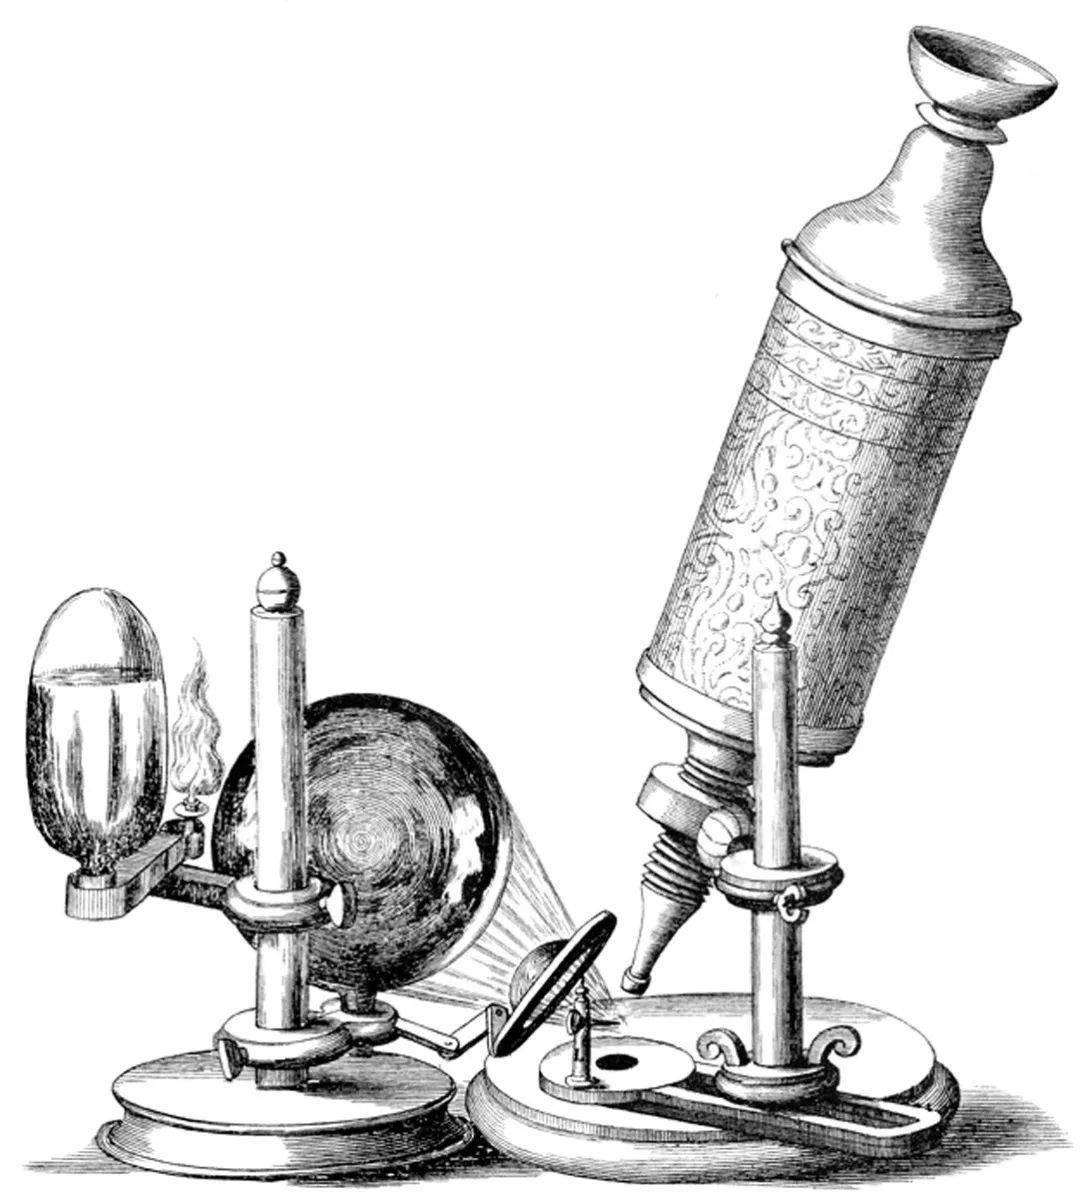
\includegraphics[width=\linewidth]{fig1.jpeg}
			\caption{Robert Hooke 制作的复合显微镜}
		\end{subfigure}%
hfill
		\begin{subfigure}{0.31\textwidth}
			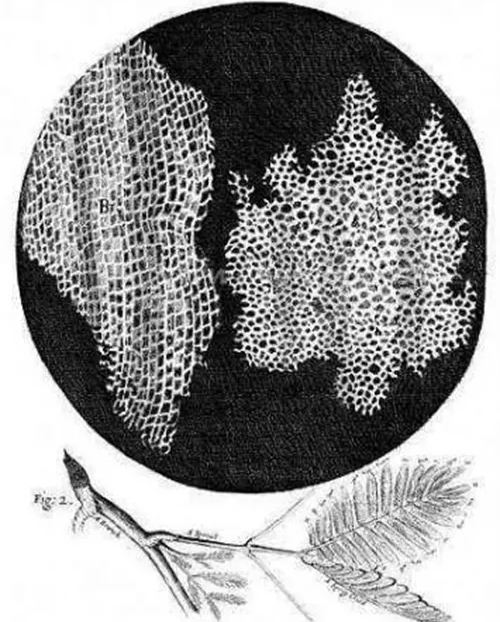
\includegraphics[width=\linewidth]{fig2.png}
			\caption{Robert Hooke 观察栎树皮薄片}
		\end{subfigure}
\hfill
		\begin{subfigure}{0.31\textwidth}
			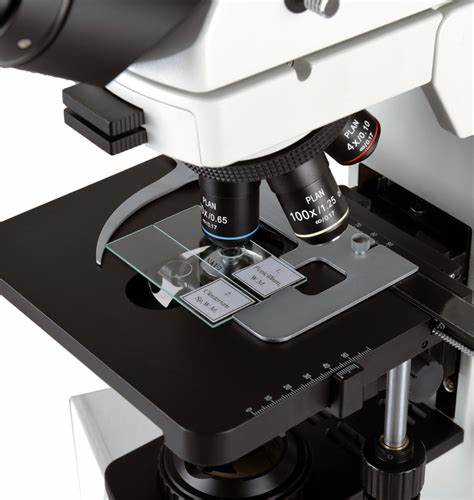
\includegraphics[width=\linewidth]{fig3.png}
			\caption{现代光学显微镜}
		\end{subfigure}
		\caption{显微镜的发展历史:光学显微镜}
	\end{figure}
	\vskip 1em

\section{用法参考}
	\subsection{伪代码}
		使用 Algorithm2e 宏包实现。

		\begin{algorithm}[H]
			\KwData{this text}
			\KwResult{how to write algorithm with \LaTeX2e }
			initialization\;
			\While{not at end of this document}{
				read current\;
				\Repeat{this end condition}{
					do these things\;
				}
				\eIf{understand}{
					go to next section\;
					current section becomes this one\;
				}{
					go back to the beginning of current section\;
				}
				\Do{this end condition}{
					do these things\;
				}
			}
			\caption{How to write algorithms}
		\end{algorithm}






\end{document}
